\chapter{Desarrollo en Arduino}\label{chp-05}

Una parte imprescindible del proyecto es la programación del propio Arduino, que es el que centraliza
todo el control del sistema. La parte relacionada con el control del motor y la programación del encoder 
está bien documentada en el trabajo \cite{tapia}, mientras que para la medición del calibre se ha partido
de la web \cite{caliper} al igual que en el diseño electrónico ya comentado en el capítulo \ref{chp-03}.

\section{Diagrama de flujo}

\begin{figure}[hbtp]
    \centering
    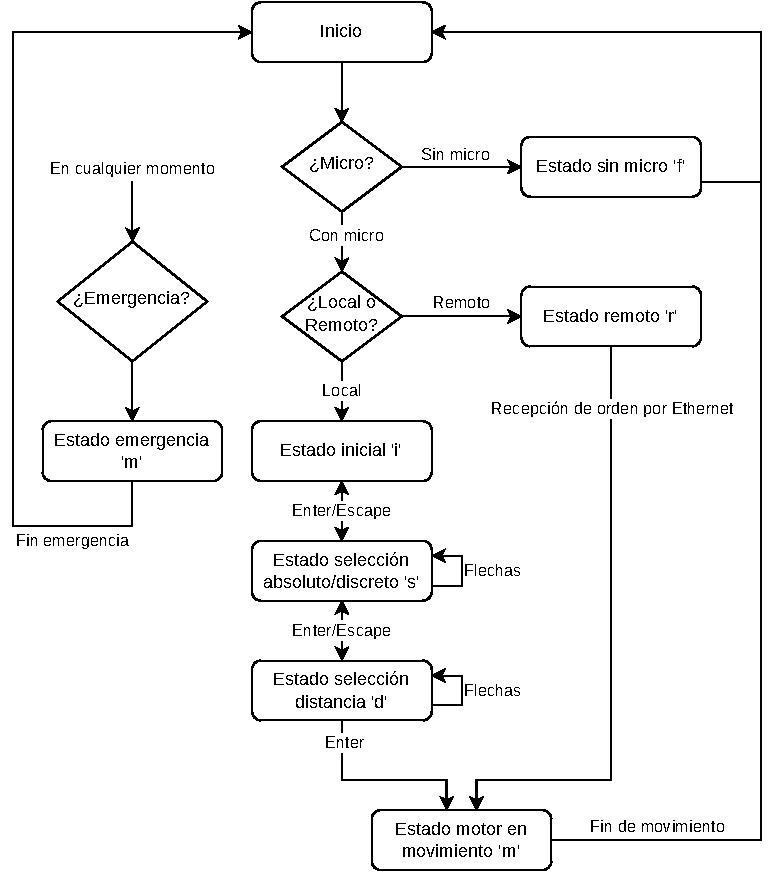
\includegraphics[height=0.5\textheight]{05-arduino/diagramaflujo.pdf}
    \caption{Diagrama de flujo del programa}
    \label{fig:diagramaflujo}
    \end{figure}

En la figura \ref{fig:diagramaflujo} se observa los distintos estados que 

\section{Programa final}

El 



\begin{lstlisting}[language=,caption={Declaración de variables, "main.h"}, breaklines=true, label=main_h]
// Definición de pines
#define faseA 2
#define faseB 3

#define BUTTON_ESC 22
#define BUTTON_ENTER 23
#define BUTTON_UP 24
#define BUTTON_DOWN 25

#define BUTTON_LOCAL 28
#define BUTTON_MICRO 29
#define BUTTON_EMERGENCIA 30

#define SENSOR_FOTO 31

#define CAL_CLK 32
#define CAL_DATA 33

#define ENB 5
#define IN3 40
#define IN4 41

// Declaración de objetos de LCD y relacionados con Ethernet
LiquidCrystal_I2C lcd(0x27,16,2);
byte MAC[] = { 0xDE, 0xAD, 0xBE, 0xEF, 0xFE, 0xED }; // Dirección MAC del dispositivo
IPAddress IP(192,168,1,200); // IP estática del dispositivo
EthernetServer servidor(4012); // Puerto donde se transmite la información

// Declaración de variables booleanas auxiliares
bool enter;
bool esc;
bool up;
bool down;
bool esc_ant = 0;
bool enter_ant = 0;
bool up_ant = 0;
bool down_ant = 0;

bool emergencia;
bool local;
bool micro;
bool fotoelectrico;

bool emergencia_ant;
bool local_ant;
bool micro_ant;

// Declaración e inicialización de variable de posición 'x' e 'y'
long posicion = 0;
long * pposicion = &posicion;
float posy = 0;

// Inicialización de variables de estado y desplazamiento
char estado = 'i';
bool discreto = 0;
long desplazamiento = 1000;
long objetivo = 0;

// Definición de parámetros de PID
float kp = 0.5;
float Ti = 2;
float Td = 0.1;
float T = 0.01;
    
\end{lstlisting}

\begin{lstlisting}[language=,caption={Código principal Arduino, "main.ino"}, breaklines=true, label=main_cpp]
// Inclusión de librerías
#include <Ethernet.h>
#include <LiquidCrystal_I2C.h>
#include "main.h"

// Definición de funciones:

// Funciones de interrupción de encoder
void cambiofaseA(void);
void cambiofaseB(void);

// Funciones relacionadas al movimiento del motor
void pararMotor(void);
void moverMotor(void);
void movimientoMotor(long objetivo, long* posicion, LiquidCrystal_I2C lcd);

// Función de lectura del calibre digital
float medidaCalibre(void);

// Funciones de conexión por Ethernet
bool comprobarRobot(void);
bool enviarRobot(char dato);
void ethconex(void);

// Función setup de configuración del sistema
void setup() {
    // Inicializar el LCD
    lcd.init();
    
    // Encender la luz de fondo.
    lcd.backlight();
    
    // Definición de pines
    pinMode(faseA, INPUT_PULLUP);
    pinMode(faseB, INPUT_PULLUP);

    pinMode(BUTTON_DOWN, INPUT);
    digitalWrite(BUTTON_DOWN, HIGH);
    pinMode(BUTTON_UP, INPUT);
    digitalWrite(BUTTON_UP, HIGH);
    pinMode(BUTTON_ENTER, INPUT);
    digitalWrite(BUTTON_ENTER, HIGH);
    pinMode(BUTTON_ESC, INPUT);
    digitalWrite(BUTTON_ESC, HIGH);

    pinMode(BUTTON_EMERGENCIA, INPUT);
    pinMode(BUTTON_LOCAL, INPUT);
    pinMode(BUTTON_MICRO, INPUT);

    pinMode(SENSOR_FOTO, INPUT);

    // En función del estado de las señales MICRO, EMER y LR la configuración de IN3, IN4 y ENB pasa a INPUT u OUTPUT para evitar conflictos
    if(!digitalRead(BUTTON_MICRO)){
    pinMode(IN3, OUTPUT);
    pinMode(IN4, OUTPUT);
    pinMode(ENB, OUTPUT);
    if(!digitalRead(BUTTON_EMERGENCIA)){
        estado = 'i';
    } else{
        estado = 'e';
    }
    if(digitalRead(BUTTON_LOCAL)){
        estado = 'r';
    }
    } else{
    pinMode(IN3, INPUT);
    pinMode(IN4, INPUT);
    pinMode(ENB, INPUT);
    estado = 'f';
    }

    // Asociación de interrupción a los pines del encoder
    attachInterrupt(digitalPinToInterrupt(faseA), cambiofaseA, RISING);
    attachInterrupt(digitalPinToInterrupt(faseB), cambiofaseB, RISING);
    
    posy = medidaCalibre();
    posicion = 0;
    // Se inicia la comunicación Ethernet y la serie para depuración
    Ethernet.begin(MAC, IP);
    Serial.begin(9600);
    Serial.print("Servidor en IP ");
    Serial.println(Ethernet.localIP());
}

// Bucle infinito
void loop() {

    // Se lee el estado de los botones
    up = digitalRead(BUTTON_UP);
    down = digitalRead(BUTTON_DOWN);
    enter = digitalRead(BUTTON_ENTER);
    esc = digitalRead(BUTTON_ESC);

    // Se lee el estado de la configuración
    emergencia = digitalRead(BUTTON_EMERGENCIA);
    local = digitalRead(BUTTON_LOCAL);
    micro = digitalRead(BUTTON_MICRO);

    // En el caso de cambio de las señales de modo o emergencia, pasar por setup() para reconfigurar los pines
    if(micro && (estado != 'f') && (estado != 'e')){
    setup();
    }

    if(local != local_ant){
    setup();
    }

    if(emergencia && (estado != 'e')){
    estado = 'e';
    lcd.clear();
    }

    // Máquina de estados
    switch(estado){
    // Estado inicial
    case 'i':
        lcd.setCursor(0, 0);
        lcd.print("MODO LOCAL      ");
        lcd.setCursor(0, 1);
        lcd.print("PULSE ENTER     ");
        digitalWrite(IN3, LOW);
        digitalWrite(IN4, LOW);
        analogWrite(ENB, 255);
        // Envío por Ethernet del estado al robot
        if(comprobarRobot()){
        enviarRobot(estado);
        }
        break;
        
    // Estado selección discreto/absoluto    
    case 's':
        lcd.setCursor(0, 0);
        lcd.print("SELECCIONE MOV. ");
        if(discreto){
        lcd.setCursor(0, 1);
        lcd.print("AVANCE DISCRETO ");
        } else{
        lcd.setCursor(0, 1);
        lcd.print("AVANCE ABSOLUTO ");
        }
        if(comprobarRobot()){
        enviarRobot(estado);
        }
        break;
        
    // Estado selección distancia de movimiento
    case 'd':
        if(comprobarRobot()){
        enviarRobot(estado);
        }
        break;
        
    // Estado movimiento del motor
    case 'm':
        if(comprobarRobot()){
        enviarRobot(estado);
        }
        movimientoMotor(objetivo, pposicion, lcd);
        if(comprobarRobot()){
        enviarRobot(estado);
        }
        posy = medidaCalibre();
        lcd.setCursor(0, 0);
        lcd.print("POSICION FINAL  ");
        lcd.setCursor(0, 1);
        lcd.print("                ");
        lcd.setCursor(0, 1);
        lcd.print("X=");
        lcd.print(posicion/10);
        lcd.print(" Y=");
        lcd.print(posy);
        delay(2000);
        estado = 'i';
        if(digitalRead(BUTTON_LOCAL)){
        estado ='r';
        }
        break;
        
    // Estado sin micro
    case 'f':
        lcd.setCursor(0, 0);
        lcd.print("SIN MICRO");
        break;
        
    // Estado emergencia
    case 'e':
        lcd.setCursor(0, 0);
        lcd.print("EMERGENCIA");
        break;
        
    // Estado remoto
    case 'r':
        lcd.setCursor(0, 0);
        lcd.print("MODO REMOTO     ");
        lcd.setCursor(0, 1);
        lcd.print("                ");
        digitalWrite(IN3, LOW);
        digitalWrite(IN4, LOW);
        analogWrite(ENB, 255);
        if(comprobarRobot()){
        enviarRobot(estado);
        }
        break;
    

    // Transiciones entre estados
    switch(estado){
    case 'i':
        if(!enter && enter_ant){
        estado = 's';
        }
        break;
        
    case 's':
        if(!enter && enter_ant){
        estado = 'd';
        
        posy = medidaCalibre();
        lcd.setCursor(0, 0);
        lcd.print("                ");
        lcd.setCursor(0, 1);
        lcd.print("                ");
        lcd.setCursor(0, 0);
        lcd.print("X=");
        lcd.print(posicion/10);
        lcd.print(" Y=");
        lcd.print(posy);

        lcd.setCursor(0, 1);
        if(desplazamiento > 0){
            lcd.print("+");
        }
        lcd.print(desplazamiento/10);
        lcd.print(" mm");                
        }
        if(!esc && esc_ant){
        estado = 'i';
        }
        if((!up && up_ant) || (!down && down_ant)){
        discreto = !discreto;
        }
        break;

    case 'd':
        if(!enter && enter_ant){
        estado = 'm';
        if(discreto){
            objetivo = posicion + desplazamiento;
        } else{
            objetivo = desplazamiento;
        }
        }
        if(!esc && esc_ant){
        estado = 's';
        }
        if(!up && up_ant){
        desplazamiento = desplazamiento + 1000;
        lcd.setCursor(0, 1);
        lcd.print("                ");
        lcd.setCursor(0, 1);
        if(desplazamiento > 0){
            lcd.print("+");
        }
        lcd.print(desplazamiento/10);
        lcd.print(" mm");        
        }
        if(!down && down_ant){
        desplazamiento = desplazamiento - 1000;
        lcd.setCursor(0, 1);
        lcd.print("                ");
        lcd.setCursor(0, 1);
        if(desplazamiento > 0){
            lcd.print("+");
        }
        lcd.print(desplazamiento/10);
        lcd.print(" mm");        
        }
        break;

    case 'f':
        if(!micro){
        setup();
        }
        break;

    case 'e':
        if(!emergencia){
        setup();
        }
        break;
    }

    // Guardado de estados
    esc_ant = esc;
    enter_ant = enter;
    up_ant = up;
    down_ant = down;
    
    emergencia_ant = emergencia;
    local_ant = local;
    micro_ant = micro;
    
    delay(10);
}

// Funciones definidas en la cabecera

// Si hay cambio en la fase A, se comprueba la fase B para definir el sentido de giro
void cambiofaseA(void){
    bool fB = digitalRead(faseB);
    if(fB){
    posicion++;
    } else{
    posicion--;
    }
}

// Si hay cambio en la fase A, se comprueba la fase B para definir el sentido de giro
void cambiofaseB(void){
    bool fA = digitalRead(faseA);
    if(fA){
    posicion--;
    } else{
    posicion++;
    }
}

// Parado de motor
void pararMotor(void){
    digitalWrite(IN3, LOW);
    digitalWrite(IN4, LOW);
    analogWrite(ENB, 255);
}

// Avance de motor a la velocidad especificada
void moverMotor(int u){
    if(u >= 0){ // Avance positivo
        digitalWrite(IN3, LOW);
        digitalWrite(IN4, HIGH);
    } else{ // Avance negativo
        digitalWrite(IN3, HIGH);
        digitalWrite(IN4, LOW);
        u = -u;
    }

    if(u > 200){
        u = 200; // La salida máxima es de 255 pero se limita a 200
    }

    analogWrite(ENB, u);
}

// Función que coloca el sistema en la posición deseada
void movimientoMotor(long objetivo, long* posicion, LiquidCrystal_I2C lcd){
    lcd.setCursor(0, 0);
    lcd.print("MOVIENDO...     ");
    lcd.setCursor(0, 1);
    lcd.print("                ");
    lcd.setCursor(0, 1);
    lcd.print((*posicion)/10);
    lcd.print("/");
    lcd.print(objetivo/10);

    long u = 0;
    long ek = 0;
    long ek1 = 0;
    long ik = 0;
    long D = 0;
    int aux = 0;
    bool emer = 0;
    
    // Bucle PID. Se mantiene buscando la posición mientras no entre dentro de un margen y la acción de control no se encuentre por debajo del umbral de funcionamiento
    while(((*posicion < objetivo - 5) || (*posicion > objetivo + 5) || (u > 55)) && !emer){
    
    emer = digitalRead(BUTTON_EMERGENCIA);

    // Se actualiza la posición actual en el LCD cada 120 ms
    aux++;
    if(aux > 3){
        lcd.setCursor(0, 1);
        lcd.print("                ");
        lcd.setCursor(0, 1);
        lcd.print((*posicion)/10);
        lcd.print("/");
        lcd.print(objetivo/10);        
        aux = 0;
    }

    //Actualización de error integral
    ek1 = ek;
    ek = objetivo - *posicion;
    ik = ik + ek;
    D = ek - ek1;
    //Cálculo de la señal de control
    u = kp * (ek + (T/Ti) * ik + (Td/T) * D);
    
    // En caso de saturación, reiniciar el error integral
    if((abs(u) > 255) && (abs(ek) > 200)){
        ik = 0;
    }

    // Limitar la acción de control al máximo que permite Arduino
    if(u > 255){
        u = 255;
    }
    if(u < -255){
        u = -255;
    }
    
    if(!emer){
        moverMotor(u);
        delay(1000 * T);
    }
    }
    
    // Parar el motor cuando se alcance la posición deseada
    pararMotor();
    
    if(emer){
    lcd.clear();
    lcd.print("EMERGENCIA");
    delay(1000*T);
    }
}

// Medida del calibre
float medidaCalibre(void){
    bool data;
    float medida;
    int value = 0;
    int signo = 0;

    unsigned long tempmicros;
    unsigned long tempmicros2;

    // Reintentar la medición hasta que se pueda realizar
    for(int j=0; j<10 && (value == 0); j++){

    tempmicros = micros();
    while (digitalRead(CAL_CLK)==LOW) {
        delayMicroseconds(1);      
    }

    tempmicros2 = micros();
    if ((tempmicros2-tempmicros)>10000) {
        // Se leen los 24 bits que proporciona el calibre
        for (int i=0; i<24; i++) {
        while (digitalRead(CAL_CLK)==HIGH) {
            delayMicroseconds(1);
        }

        data = !digitalRead(CAL_DATA);
    
            // Se leen los datos cada bajada del flanco de reloj
        if(i<16){
            value |= data << i;
        }else{
            signo |= (data << (i-16));
        }

        while (digitalRead(CAL_CLK)==LOW) {
            delayMicroseconds(1);
        }
        }
        
        // El bit 0x80 corresponde a las unidades, pulgadas o milímetros
        // En caso de que sean pulgadas, se realiza la conversión a milímetros
        if(signo & 0x80){
        medida = 25.4*float(value)/(2*1000);
        } else{
        medida = float(value)/100;
        } 

        // El bit 0x10 corresponde al signo
        if(signo & 0x10){
        medida = -medida;
        }
    }
    }
    return medida;
}

// Comprobación de que existe una conexión con el robot
// Devuelve 1 si se produce la conexión y 0 en caso contrario
bool comprobarRobot(void){
    EthernetClient cliente = servidor.available();
    if (cliente) {
    return 1;
    } else{
    cliente.stop();
    return 0;
    }
}

// Función para enviar estado del sistema, sensor fotoélectrico y recibir la orden de movimiento del propio robot
// El robot envía la orden, ya sea de recibir el estado del sistema o el movimiento deseado
// Una vez recibido, el Arduino envía los datos necesarios y mueve la cinta si se encuentra en estado remoto
bool enviarRobot(char dato){
    EthernetClient cliente = servidor.available();
    String recepcion;
    if (cliente) {
    while (cliente.connected()) {
        if (cliente.available()) {
        recepcion = cliente.readString();
        Serial.println(recepcion);
        if(recepcion == "STATUS"){
            String envio = (String) dato + ";X=" + String(posicion, 2) + ";Y=" + String(posy, 2);
            String fotoele = ";F=" + String(digitalRead(SENSOR_FOTO));
            envio = envio + fotoele;
            cliente.println(envio);
            Serial.println(recepcion);
        }
        if(recepcion.indexOf('M') > -1){
            if(estado == 'r'){
            int igual_pos = recepcion.indexOf("=");
            int fin_pos = recepcion.indexOf(";",igual_pos);
            String movimiento = recepcion.substring(igual_pos+1, fin_pos);
            objetivo = movimiento.toInt();
            estado = 'm';
            }
        }
        if(recepcion.indexOf('R') > -1){
            if(estado == 'r'){
            int igual_pos = recepcion.indexOf("=");
            int fin_pos = recepcion.indexOf(";",igual_pos);
            String movimiento = recepcion.substring(igual_pos+1, fin_pos);
            objetivo = movimiento.toInt() + posicion;
            estado = 'm';
            }
        }
        }
    }
    cliente.stop();
    }
    return 0;
}    
\end{lstlisting}